\title{Implementing a MIPS processor using SME}
\author{Carl-Johannes Johnsen (grc421)}
%% Skabelon til LiCS-afleveringer

%%%%%%%%%%%%%%%%%%%%%%%%%%%%%%%%%%%%%%%%%%%%%%%%%%%%%%%%%%%%%%%
%% Begynd preamble
%%%%%%%%%%%%%%%%%%%%%%%%%%%%%%%%%%%%%%%%%%%%%%%%%%%%%%%%%%%%%%%
\documentclass[a4paper]{article}

%% Til at tegne træer!
\usepackage{tikz}
\usetikzlibrary{positioning,arrows,calc}
\tikzset{
    on grid,
    node distance=3cm,
    auto,
    block/.style = {
        draw,
        shape=rectangle,
        minimum height=3em,
        minimum width=3em,
        line width=1pt
    },
    control/.style = {
        draw,
        shape=circle,
        minimum height=7em,
        minimum width=3em,
        line width=1pt
    },
    mux/.style = {
        draw,
        shape=rectangle,
        minimum height=1.5em,
        minimum width=1em,
        line width=1pt
    },
    empty/.style = {
        shape=rectangle,
        minimum height=3em,
        minimum width=3em
    },
    >=latex',
}

%% Til at kunne have billeder
\usepackage{graphicx}
%% Til at kunne have source code
\usepackage{listings}
\lstset{
  breaklines=true,
  keepspaces=true,
  frame=ltrb,
  framesep=1pt,
  commentstyle=\color{Brown},
  basicstyle=\ttfamily\footnotesize,
  numbers=left,
  title=\lstname,
  columns=fullflexible,
  extendedchars=\true,
  inputencoding=ansinew,
}

%% Font and input encoding
%% Tillad æøå
\usepackage[T1]{fontenc}
\usepackage[utf8x]{inputenc}
%% Babel (language)
\usepackage[UKenglish]{babel} % If you write in English
\usepackage[UKenglish]{isodate}
%\usepackage{parskip}
\usepackage{booktabs}
%\usepackage[danish]{babel} % Hvis du skriver på dansk

%% Til links
\usepackage{hyperref}
\usepackage{subfig}

%% AMS-Math packages
\usepackage{amsmath}
\usepackage{amssymb}
\usepackage{amsthm}
\newtheorem{theorem}{Theorem}
%% Extra symbols that we almost always need
\usepackage{stmaryrd}
\usepackage{color}
\usepackage{url}
\usepackage{semantic}
\usepackage{fancyref}
\usepackage{enumitem}

%%%%%%%%%%%%%%%%%%%%%%%%%%%%%%
%% Skift sidenumrene ud med X/total (lettere at rette :-)
\usepackage{lastpage}
\makeatletter
\renewcommand{\@oddfoot}{\hfil \thepage{}/\pageref{LastPage} \hfil}
\renewcommand{\@evenfoot}{\hfil \thepage{}/\pageref{LastPage} \hfil}
\makeatother
%%%%%%%%%%%%%%%%%%%%%%%%%%%%%%

% Til klasse diagrammer
\usepackage{pgf-umlcd}
\renewcommand{\umldrawcolor}{black}
\renewcommand{\umlfillcolor}{white}
\let\classoperation\operation

% forkortelse af texttt!
\renewcommand{\bf}{\textbf}
\renewcommand{\tt}{\texttt}
\renewcommand{\sf}{\textsf}
\renewcommand{\it}{\textit}
\newcommand{\E}{\mathbb{E}}

% Forkortelser som bruger tt!
\newcommand{\tif}{\tt{ if }}
\newcommand{\tthen}{\tt{ then }}
\newcommand{\telse}{\tt{ else }}
\newcommand{\tfalse}{\tt{ false }}

%%%%%%%%%%%%%%%%%%%%%%%%%%%%%%%%%%%%%%%%%%%%%%%%%%%%%%%%%%%%%%%
%% Slut preamble -- herunder følger selve dokumentet!
%%%%%%%%%%%%%%%%%%%%%%%%%%%%%%%%%%%%%%%%%%%%%%%%%%%%%%%%%%%%%%%
\sloppy
\begin{document}
\maketitle

\begin{abstract}
asoenuthnsoaeuhtt
\end{abstract}


\newpage
\tableofcontents
\newpage

\section{Introduction}
\subsection{Software requirements for using SME}
SME is a library for \tt{C\#}. Therefor we need to setup a development
environment for \tt{C\#}. We will be using \tt{mono} URL % TODO

Now that we have \tt{mono} installed, we need to download and run \tt{SME}. We
start by cloning the project from github: URL!. % TODO
Then, we add the project in
\tt{monodevelop}. Before building the project, we need to generate a few files
(\tt{SME.Render.VHDL/Entity.tt} and \tt{SME.Render.VHDL/TopLevel.tt},
which is done by right clicking the file, and choosing 'Tools > Process T4
Template'. Finally, we can open one of the example programs, and press f5 to
build and run.

%install monodevelop
%clone from github
%run process T4 template on SME.Render.VHDL/Entity.tt and
%SME.Render.VHDL/TopLevel.tt
%Open example project, and press f5 to build and run

\subsection{Logic gates}
To start with, I am going to implement the 4 basic logic gates: \tt{AND},
\tt{OR}, \tt{NOT} and \tt{XOR}, as these are the basic building blocks of a
processor.

I start by describing the busses. I have one input bus, which has two fields:
\tt{Bit1} and \tt{Bit2}, and an output bus, which has four fields, one for each
gate. Note that these interfaces has to be public
%%\lstinputlisting{Buses.cs}

Then I define the processes for each of the logic gates. They are very simple,
as they just take the two inputs, applies their logic operation, and puts the
output on the designated lane on the output bus.
%\lstinputlisting{Gates.cs}

Finally, I wrote a test process, which feeds input to the gate processes,
stores the output from the gate processes, and finally verifies the collected
results, which is:
\begin{tabular}{cc|cccc}
    \tt{Bit1} & \tt{Bit2} & \tt{AND} & \tt{OR} & \tt{NOT} & \tt{XOR} \\
    \hline
    false     & false     & false    & false   & true     & false \\
    false     & true      & false    & true    & true     & true  \\
    true      & false     & false    & true    & false    & true  \\
    true      & true      & true     & true    & false    & false \\
    \hline
\end{tabular}
%\lstinputlisting{GateTester.cs}

\subsection{Decoder}
A decoder takes an $n$-bit input, and has $2^n$ outputs. Exactly one of the
outputs are \tt{1} on any given input. If the value of the input is \tt{0}, then
bit0 of the output is set to \tt{1}, and the rest is set to \tt{0}. If the
value of the input is 124, then bit124 is set to \tt{1}, and the rest is set to
\tt{0}.

I have implemented a 2-bit encoder, by having 2 \tt{NOT} gates, and 4 \tt{AND}
gates:
% TODO figurer!!!

\subsection{Scalable Decoder}
The previous decoder was a hardcoded decoder, i.e. that I had manually defined
all of the busses and the processes. Since SME requires that everything is
known at compile time, we have to define everything statically. This results in
an exponential amount of work when making a larger decoder, where the work is
primarely defining the buses, each has to have an unique name, and defining the
processes, as each has to read from a different bus, or in another case, read
from a different wire on the bus.

To solve this, I have used T4 Templates to generate the source code files for
me, since the network is just a bunch of busses, \tt{NOT} gates and \tt{AND}
gates.

\subsection{Half adder}
A half adder is a circuit, which takes 2 inputs, each one bit, and adds them
together, outputting a sum bit and a carry bit.

\subsection{Full adder}
A full adder is a circuit, which takes 3 inputs, each one bit, and adds them
together, outputting a sum bit, and a carry bit. The difference between a half
adder and a full adder is the extra input, which is designated to be the carry
from the previous full adder in a chain of adders.

\subsection{32 bit adder}
Now that I have made scalable \tt{SME} networks, an half adder and a full
adder, I can make a 32 bit adder. The 32 bit adder starts with an half adder
connected to the first bit of the first input number and to the first bit of
the second input number. The output of the half adder is the first bit of the
output. The remainder of the adder consists of 31 full adders, where we say
that the $i$th full adder is connected to the $i$th bit of both of the input
numbers, to the carry from the $i-1$th adder, and outputs the $i$th bit of the
result, and the $i$th carry. The last carry is the flag indicating whether or
not the addition produced an overflow.

I have made the implementation using Templates, and as such, we can also use
this to produce an $n$-bit adder, just by changing the \tt{BitWidth} variable
of each of the template files.


% Remember! newpage on new chapters
\newpage
\section{Getting started with SME}
\subsection{Installing SME}
\subsection{Writing first SME program}
\subsection{C\# and bit hacking}
\subsection{Translating first SME program into VHDL}
\subsection{Running and verifying VHDL}


\newpage
\section{Basic logic circuits}
\label{sec:logic-circuits}
In this section, I will be looking at some basic combinatorial circuits. I
start by looking at some logic gates, which implement some boolean functions.
% TODO: omskriv vil jeg mene!
All of the considered values in the system are binary, e.g. the logic gates
works on \texttt{1}s and \texttt{0}s.

\subsection{Basic logic gates}
Start by defining the basic logic gates, which are common for most circuits. A
logic gate is a circuit abstraction, which has inputs and outputs. Its output
values are based upon the input values.

\begin{description}
    \item[\texttt{AND}] - outputs \texttt{1} iff. all of its inputs are
        \texttt{1}, otherwise it outputs \texttt{0}.

    \item[\texttt{OR}] - outputs \texttt{1} if one or more of its inputs are
        \texttt{1}, otherwise it outputs \texttt{0}.

    \item[\texttt{NOT}] -outputs the inverse of its input, i.e. \texttt{1}
        becomes \texttt{0} and \texttt{0} becomes \texttt{1}.

    \item[\texttt{XOR}] - outputs \texttt{1} iff exactly one of its inputs are
        \texttt{1}, otherwise it outputs \texttt{0}
\end{description}
The full truth table for all of the four logic gates can be seen in Table
\ref{tab:truth-table}

\begin{table}
    \centering
    \begin{tabular}{cc|cccc}
        \toprule
        \texttt{Bit1} & \texttt{Bit2} & \texttt{AND} & \texttt{OR} &
        \texttt{NOT} & \texttt{XOR} \\
        \midrule
        false     & false     & false    & false   & true     & false \\
        false     & true      & false    & true    & true     & true  \\
        true      & false     & false    & true    & false    & true  \\
        true      & true      & true     & true    & false    & false \\
        \bottomrule
    \end{tabular}
    \caption{The truth table for the four basic logic gates. Note: \texttt{NOT}
    is only considering \texttt{Bit1}.}
    \label{tab:truth-table}
\end{table}

\subsubsection{Implementation}
Implementing each of these four logic gates is quite simple: There is an input
bus with two 1-bit values, a process for each of the gates, and an output bus
with a 1-bit value for each of the logic gates. % (See Figure
%\ref{fig:logic-gate}).
%
%\begin{figure}
%    \centering
%    \begin{tikzpicture}
%        \coordinate(input);
%        \node[block, right of=input] (A) {Logic gate};
%        \path[->] (input) edge node [midway, above] {input} (A);
%        \node[right of=A] (output) {};
%        \path[->] (A) edge node [midway, above] {output} (output);
%    \end{tikzpicture}
%    \caption{The structure of a Logic gate process}
%    \label{fig:logic-gate}
%\end{figure}

\subsubsection{Testing}
To test the four processes, I have made a process, which sets the bits to all
of the values in the truth table, and checks whether or not each process
outputs the expected value from the truth table. How the processes are
connected can be seen in Figure \ref{fig:logic-test}.

\begin{figure}
    \centering
    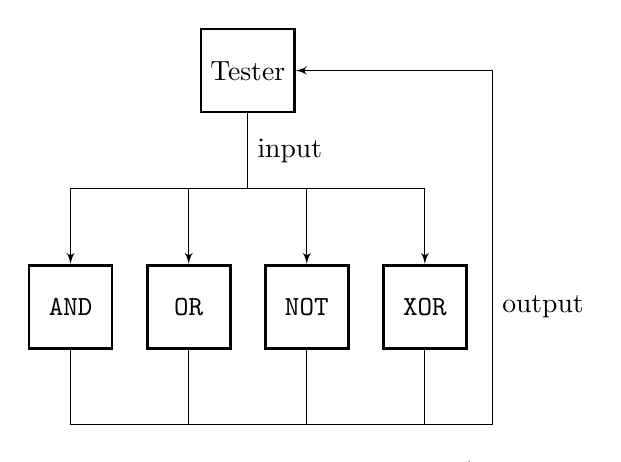
\begin{tikzpicture}[node distance=1.5cm]
        \node[block] (and) {\texttt{AND}};
        \node[block, right of=and] (or) {\texttt{OR}};
        \node[block, right of=or] (not) {\texttt{NOT}};
        \node[block, right of=not] (xor) {\texttt{XOR}};
        \node[above of=and] (input) at ($(or)!0.5!(not)$) {};
        \node[block, above of=input] (tester) {Tester};

        \path[-] (tester) edge node[midway, right] {input} (input.center);
        \path[draw, ->] (input.center) -| (and.north);
        \path[draw, ->] (input.center) -| (or.north);
        \path[draw, ->] (input.center) -| (not.north);
        \path[draw, ->] (input.center) -| (xor.north);

        \node[below of=and] (output) at ($(or)!0.5!(not)$) {};
        \node[right of=xor] (a) {output};

        \path[draw, -] (and.south) |- (output.center);
        \path[draw, -] (or.south) |- (output.center);
        \path[draw, -] (not.south) |- (output.center);
        \path[draw, -] (xor.south) |- (output.center);

        \path[draw, -] (output.center) -| (a.west);
        \path[draw, ->] (a.west) |- (tester.east);
    \end{tikzpicture}
    \caption{The structure of the test of the logic gates}
    \label{fig:logic-test}
\end{figure}

\subsection{Decoder}
% TODO 0-indexed!
The first combinatorial circuit I make is the decoder. An decoder takes an
$n$-bit input, and produces an $2^n$-bit output, where the bit corresponding to
the input numbers value is set to \texttt{1}. E.g. if the input value is the
binary representation of the number 5, then the 5th output bit will be
\texttt{1}, and the rest will be \texttt{0}.

A decoder can be made from a set of \texttt{NOT} and \texttt{AND} gates. We
need to have $n$ \texttt{NOT} gates, and $2^n$ \texttt{AND} gates. For each
input, we split it into two, and send the copy to a \texttt{NOT} gate. Then for
each output, we attach an \texttt{AND} gate, and give it inputs corresponding
to the binary representation of the number %TODO mangler ord.
E.g. if we get the number 5, the binary representation is 101, i.e. the 5th
\texttt{AND} gate gets input from Bit0, \texttt{NOT} Bit1 and Bit2. An example
of a 2-bit decoder can be seen in Figure \ref{fig:2-bit-decoder}.

\begin{figure}
    \centering
    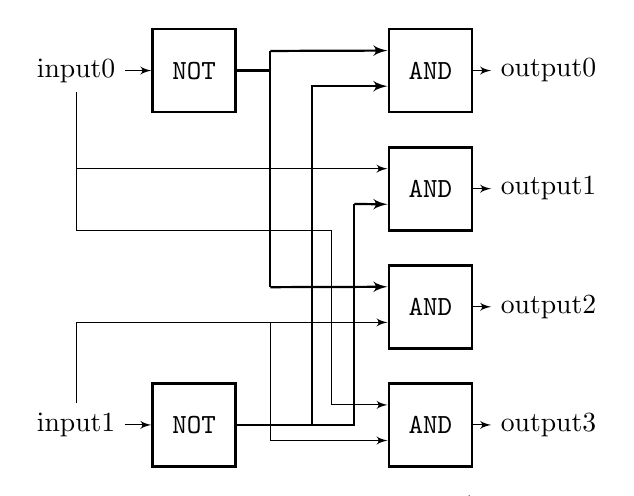
\begin{tikzpicture}[node distance=1.5cm]
        \node[block] (and0) {\texttt{AND}};
        \node[block, below of=and0] (and1) {\texttt{AND}};
        \node[block, below of=and1] (and2) {\texttt{AND}};
        \node[block, below of=and2] (and3) {\texttt{AND}};

        \node[right of=and0] (output0) {output0};
        \node[right of=and1] (output1) {output1};
        \node[right of=and2] (output2) {output2};
        \node[right of=and3] (output3) {output3};

        \path[draw, ->] (and0) -- (output0);
        \path[draw, ->] (and1) -- (output1);
        \path[draw, ->] (and2) -- (output2);
        \path[draw, ->] (and3) -- (output3);

        \node[empty, left of=and0] (andinp0) {};
        \node[empty, left of=and1] (andinp1) {};
        \node[empty, left of=and2] (andinp2) {};
        \node[empty, left of=and3] (andinp3) {};

        \node[block, left of=andinp0] (not0) {\texttt{NOT}};
        \node[block, left of=andinp3] (not1) {\texttt{NOT}};

        \node[left of=not0] (input0) {input0};
        \node[left of=not1] (input1) {input1};

        \path[draw, ->] (input0) -- (not0);
        \path[draw, ->] (input1) -- (not1);

        \path[draw, thick, -] (not0) -| (andinp0.155);
        \path[draw, thick, ->] (andinp0.155) -- (and0.155);
        \path[draw, thick, -] (not1.east) -| (andinp0.south);
        \path[draw, thick, ->] (andinp0.south) |- (and0.200);

        \path[draw, ->] (input0) |- (and1.155);
        \path[draw, thick, -] (not1.east) -| (andinp1.340);
        \path[draw, thick, ->] (andinp1.340) -- (and1.200);

        \path[draw, thick, -] (not0.east) -| (andinp2.155);
        \path[draw, thick, ->] (andinp2.155) -- (and2.155);
        \path[draw, ->] (input1.north) |- (and2.200);

        \path[draw, -] (input0) |- (andinp1.295);
        \path[draw, ->] (andinp1.295) |- (and3.155);
        \path[draw, -] (input1) |- (andinp2.200);
        \path[draw, ->] (andinp2.200) |- (and3.200);

    \end{tikzpicture}
    \caption{An 2-bit decoder made by \texttt{AND} and \texttt{NOT} gates.}
    \label{fig:2-bit-decoder}
\end{figure}

%\subsubsection{$n$-bit decoder}
\subsubsection{Testing}
I have written both a 2-bit decoder, and an $n$-bit decoder. They are tested in
the same fashion as the logic gates, i.e. a tester process is connected to the
input and output bus. The test inputs every combination of numbers, i.e. $2^n$,
and checks after each input, that the correct output is set to \texttt{1} and
\texttt{0} respectively.

\subsection{Adder}
As with the decoder, an adder can be constructed by a combination of
\texttt{AND}, \texttt{OR} and \texttt{XOR} gates. An $n$-bit adder is a chain
of two major components: an half adder and a full adder.

The half adder is the initial component in the chain. It takes two binary
inputs, and outputs the sum and the carry of the addition (See Figure
\ref{fig:half-adder}.

The rest of the $n$-bit adder consists of a chain of full adders, that take
three inputs, A, B, and the carry from the previous link in the chain, and
outputs the sum and the carry of the addition (See Figure
\ref{fig:full-adder}).

The combination of the components can be seen in Figure \ref{fig:n-bit-adder}.


\begin{figure}
    \centering
    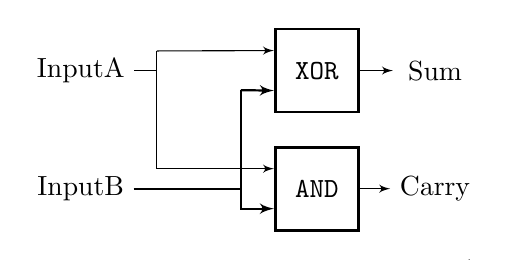
\begin{tikzpicture}[node distance=1.5cm]
        \node[block] (xor) {\texttt{XOR}};
        \node[block, below of=xor] (and) {\texttt{AND}};

        \node[empty, left of=xor] (xorin) {};
        \node[empty, left of=and] (andin) {};

        \node[left of=xorin] (inputa) {InputA};
        \node[left of=andin] (inputb) {InputB};

        \node[empty, right of=xor] (sum) {Sum};
        \node[empty, right of=and] (carry) {Carry};

        \path[draw, -] (inputa) -| (xorin.155);
        \path[draw, ->] (xorin.155) -- (xor.155);
        \path[draw, ->] (xorin.west) |- (and.155);

        \path[draw, thick, -] (inputb.east) -| (xorin.335);
        \path[draw, thick, ->] (xorin.335) -- (xor.205);
        \path[draw, thick, ->] (andin.east) |- (and.205);

        \path[draw, ->] (xor) -- (sum);
        \path[draw, ->] (and) -- (carry);
    \end{tikzpicture}
    \caption{An half adder composed of \texttt{XOR} and \texttt{AND} gates}
    \label{fig:half-adder}
\end{figure}

\begin{figure}
    \centering
    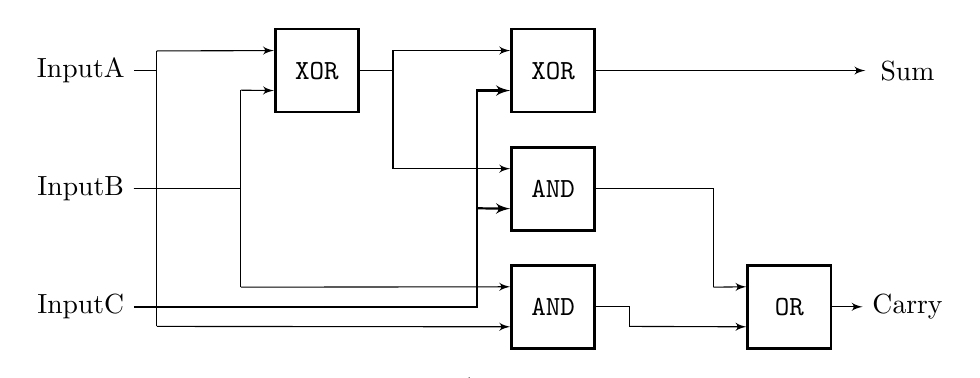
\begin{tikzpicture}[node distance=1.5cm]
        \node[block] (or) {\texttt{OR}};
        \node[empty, left of=or] (orin) {};
        \node[block, left of=orin] (and1) {\texttt{AND}};
        \node[block, above of=and1] (and0) {\texttt{AND}};
        \node[empty, left of=and0] (and0in) {};
        \node[block, above of=and0] (xor1) {\texttt{XOR}};
        \node[empty, left of=xor1] (xor1in) {};
        \node[block, left of=xor1in] (xor0) {\texttt{XOR}};
        \node[empty, left of=xor0] (xor0in) {};
        \node[empty, left of=xor0in] (inputa) {InputA};
        \node[empty, below of=inputa] (inputb) {InputB};
        \node[empty, below of=inputb] (inputc) {InputC};
        \node[empty, right of=inputc] (inputcout) {};
        \node[empty, right of=xor1] (sum) {};
        \node[empty, right of=sum] (summ) {};
        \node[empty, right of=summ] (summm) {Sum};
        \node[empty, right of=or] (carry) {Carry};

        \path[draw, -] (inputa.east) -| (xor0in.155);
        \path[draw, ->] (xor0in.155) -- (xor0.155);
        \path[draw, -] (inputb.east) -| (xor0in.335);
        \path[draw, ->] (xor0in.335) -- (xor0.205);

        \path[draw, -] (inputa.east) -| (inputcout.205);
        \path[draw, ->] (inputcout.205) -- (and1.205);
        \path[draw, -] (inputb.east) -| (inputcout.25);
        \path[draw, ->] (inputcout.25) -- (and1.155);

        \path[draw, thick, -] (inputc.east) -| (and0in.335);
        \path[draw, thick, ->] (and0in.335) -- (and0.205);
        \path[draw, thick, ->] (and0in.335) |- (xor1.205);

        \path[draw, -] (xor0.east) -- (xor1in.west);
        \path[draw, ->] (xor1in.west) |- (xor1.155);
        \path[draw, ->] (xor1in.west) |- (and0.155);

        \path[draw, -] (and1.east) -| (orin.205);
        \path[draw, ->] (orin.205) -- (or.205);
        \path[draw, ->] (xor1) -- (summm);
        \path[draw, -] (and0.east) -| (orin.25);
        \path[draw, ->] (orin.25) -- (or.155);
        \path[draw, ->] (or) -- (carry);
    \end{tikzpicture}
    \caption{A full adder composed of \texttt{AND}, \texttt{OR} and
    \texttt{XOR} gates}
    \label{fig:full-adder}
\end{figure}

\begin{figure}
    \centering
    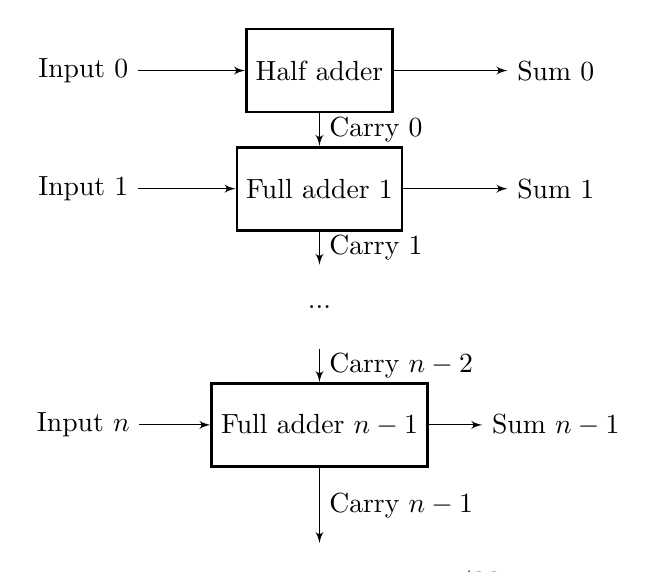
\begin{tikzpicture}[node distance=1.5cm]
        \node[block] (half) {Half adder};
        \node[block, below of=half] (full1) {Full adder 1};
        \node[empty, below of=full1] (dot) {...};
        \node[block, below of=dot] (fulln) {Full adder $n-1$};

        \node[empty, left of=half] (spacingl) {};
        \node[empty, right of=half] (spacingr) {};

        \node[empty, left of=spacingl] (in0) {Input 0};
        \node[empty, below of=in0] (in1) {Input 1};
        \node[empty, below of=in1] (vertspacel) {};
        \node[empty, below of=vertspacel] (inn) {Input $n$};

        \node[empty, right of=spacingr] (out0) {Sum 0};
        \node[empty, below of=out0] (out1) {Sum 1};
        \node[empty, below of=out1] (vertspacer) {};
        \node[empty, below of=vertspacer] (outn) {Sum $n-1$};
        \coordinate[below of=fulln] (carry);

        \path[draw, ->] (in0) -- (half);
        \path[draw, ->] (in1) -- (full1);
        \path[draw, ->] (inn) -- (fulln);

        \path[draw, ->] (half) -- (out0);
        \path[draw, ->] (full1) -- (out1);
        \path[draw, ->] (fulln) -- (outn);

        \path[draw, ->] (half) -- node [midway, right] {Carry 0} (full1);
        \path[draw, ->] (full1) -- node [midway, right] {Carry 1} (dot);
        \path[draw, ->] (dot) -- node [midway, right] {Carry $n-2$} (fulln);
        \path[draw, ->] (fulln) -- node [midway, right] {Carry $n-1$} (carry);
    \end{tikzpicture}
    \caption{An $n$-bit adder composed of a half adder, and $n-1$ full adders.
    Note: Input A and B are both inside the inputs for simplicity.}
    \label{fig:n-bit-adder}
\end{figure}

\subsubsection{Testing}
I have tested both the half adder and the full adder, by giving each every
possible input, and for each, compared them to their expected output. For the
$n$-bit adder, I have made a function, that takes an integer as input, sends it
along the corresponding input wires. I have also made a similar function, that
takes the values from the output wires and packs it into an integer. I start by
testing if it can make one of the simplest additions: 2+2. Then I check if it
can overflow, i.e. set the Carry $n-1$ to \texttt{1}. Finally, I run a series
of random numbers through the adder, and check if the output is the expected
sum of the two numbers.


\newpage
\section{Core components}
\subsection{Register file}
The register file is the component that holds values for the processor. It is
the first step in a memory hierarchy, and thus the fastest memory available.
There are 32 registers in a 32-bit MIPS processor. The registers are devided
into groups based on their usage. This does not matter from a hardware
perspective, except for register 0, which is immutable and always 0.

A register file has 5 inputs: Read address A, Read address B, Write enabled,
Write address and Write data. It also has two outputs: Output A and Output B.
We need to be careful of the order in which we read and write from the register
file. We need to make sure that when an instruction reads from the register
file, it always gets the latest data, i.e. if an instruction reads from the
same register as a previous instruction writes to, it should get the written
value. This is easy to fix in the single cycle processor, as we just need to
write before reading.

\begin{figure}
    \centering
    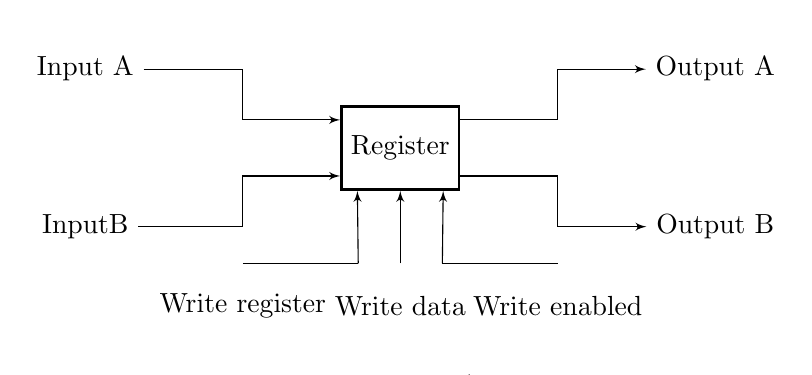
\begin{tikzpicture}[node distance=2cm]
        \node[empty] (inputa) {Input A};
        \node[empty, below of=inputa] (inputb) {InputB};

        \node[empty, right of=inputa] (spacing) at ($(inputa)!0.5!(inputb)$) {};
        \node[block, right of=spacing] (register) {Register};
        \node[empty, below of=register] (writedata) {Write data};
        \node[empty, left of=writedata] (write) {Write register};
        \node[empty, right of=writedata] (writeenabled) {Write enabled};

        \node[empty, right of=inputa] (space) {};
        \node[empty, right of=space] (spacee) {};
        \node[empty, right of=spacee] (spaceee) {};
        \node[empty, right of=spaceee] (outputa) {Output A};
        \node[empty, below of=outputa] (outputb) {Output B};
        \node[empty, left of=outputb] (bspace) {};

        \path[draw, -] (inputa) -| (spacing.north);
        \path[draw, ->] (spacing.north) |- (register.155);
        \path[draw, -] (inputb) -| (spacing.south);
        \path[draw, ->] (spacing.south) |- (register.205);

        \path[draw, -] (write) |- (writedata.135);
        \path[draw, ->] (writedata.135) -- (register.225);
        \path[draw, ->] (writedata) -- (register);
        \path[draw, -] (writeenabled) |- (writedata.45);
        \path[draw, ->] (writedata.45) -- (register.315);

        \path[draw, -] (register.335) -| (bspace.north);
        \path[draw, ->] (bspace.north) |- (outputb);
        \path[draw, -] (register.25) -| (spaceee.south);
        \path[draw, ->] (spaceee.south) |- (outputa);
    \end{tikzpicture}
    \caption{The register file}
    \label{fig:register}
\end{figure}

\bf{Testing} - I start by testing if some of the initial values of the register
file is correctly set to 0. Then I test if I can write to a register, and
whether or not I can read the same value from the same address in the register.
Then, I try to write to all of the registers, except for 0, and check whether
or not the output that I get, corresponds with the output that I wrote.

\subsection{ALU}
The ALU (Arithmetic Logic Unit) is the part of the processor, which makes the
actual computation. It takes three inputs: InputA, InputB and an ALU opcode
indicating which computation to perform. It has two outputs: The result of the
computation, and a zero flag indicating whether or not the result of the
computation was 0.

I follow the approach from the book % TODO ref!
and have implemented the basic processor operations: \texttt{add}, \texttt{sub},
\texttt{and}, \texttt{or} and \texttt{slt} (set less than).

I have tested each of the four operations.


% TODO ! husk at man kan bruge ghostscript (gs) til compression!
\newpage
\section{Single cycle MIPS processor}
In this section, we will be combining the core components into a single cycle
MIPS processor, i.e. a processor where exactly one instruction is executed per
clock cycle. When it is in place, we will be writing the first program, and
compiling it into the processor, and running it.

Following the single cycle MIPS processor, we will be extending
the processor so that it can handle more instructions. Along each added
instruction, we will be extending our first program, in order to verify that
the instruction works.

Finally, we will be writing two programs, and look into compiling them into a
series of hex values, that we can copy straight into the Instruction Memory.

\subsection{Wiring up the processor}
\begin{figure}
    \centering
    \scalebox{0.5}{
        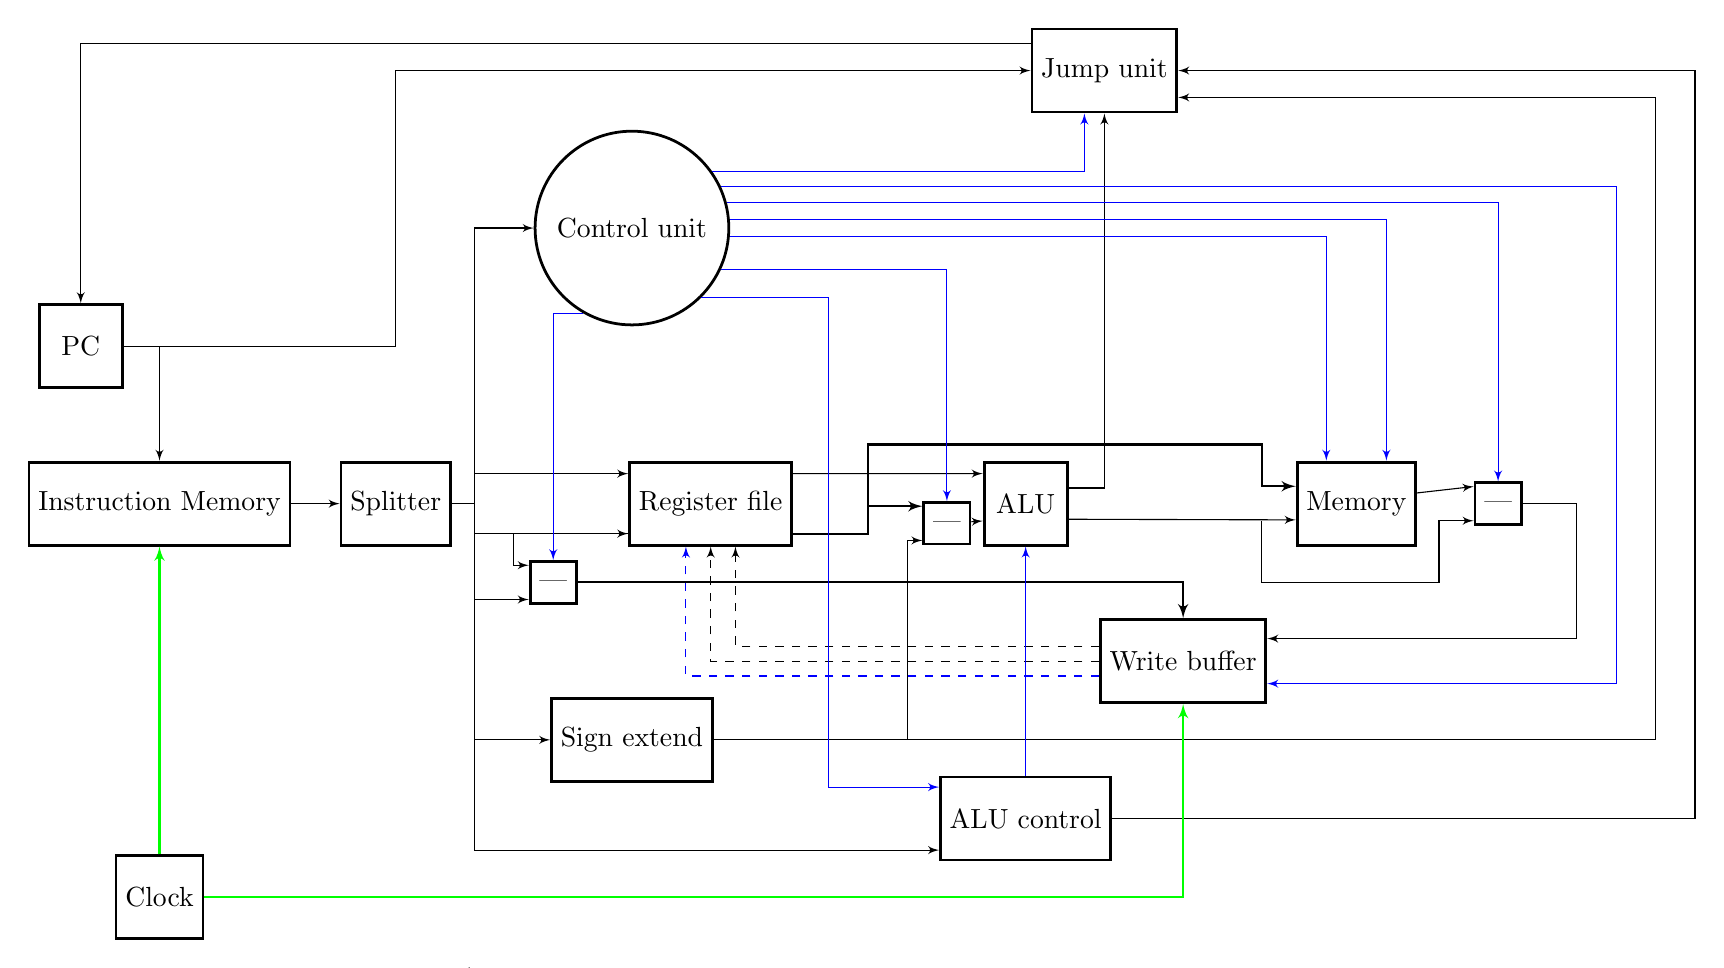
\begin{tikzpicture}
            \node[block] (reg) at (0,0) {Register file};
            \node[control] (cont) at (-1,3.5) {Control unit};
            \node[block] (jump) at (5,5.5) {Jump unit};
            \node[empty] (splitspace) at (-3,0) {};
            \node[block] (split) at (-4,0) {Splitter};
            \node[block] (if) at (-7,0) {Instruction Memory};
            \node[block] (sign) at (-1,-3) {Sign extend};
            \node[block] (alu) at (4,0) {ALU};
            \node[block] (alucont) at (4,-4) {ALU control};
            \node[block] (mem) at (8.2,0) {Memory};
            \node[mux] (memread) at (10,0) {|};
            \node[mux] (imm) at (3, -0.25) {|};
            \node[mux] (regdst) at (-2,-1) {|};
            \node[block] (pc) at (-8, 2) {PC};
            \node[block] (writebuf) at (6, -2) {Write buffer};

            \path[draw, ->] (if) -- (split);
            \path[draw, -] (split) -- (splitspace.center);
            \path[draw, ->] (splitspace.center) |- (sign);
            \path[draw, ->] (splitspace.center) |- (cont);
            \path[draw, ->] (splitspace.center) |- (reg.160);
            \path[draw, ->] (splitspace.center) |- (reg.200);
            \path[draw, ->] (splitspace.center) |- (alucont.200);
            \path[draw, ->] (splitspace.center) |- (regdst.215);
            \path[draw, ->] (reg.200) -| (-2.5, -0.5) |- (regdst.145);
            \path[draw, ->] (alucont) -| (12.5, 0) |- (jump);
            \path[draw, thick, ->] (reg.340) -| (2,-0.25) |- (imm.145);
            \path[draw, thick, ->] (2,-0.25) |- (3,0.75) -- (7,0.75) |-
            (mem.164);
            \path[draw, ->] (reg.20) -- (alu.145);
            \path[draw, ->] (alu.20) -| (jump);
            %\path[draw, ->] (alu.340) -- (jal);
            %\path[draw, ->] (jal) -- (mem.196);
            %\path[draw, ->] (jal) -- (writebuf);
            \path[draw, ->] (alu.340) -- (mem.195);
            \path[draw, ->] (imm) -- (alu.202);
            \path[draw, ->] (7, -0.22) |- (8, -1) -| (9.25,-0.5) |-
            (memread.215);
            \path[draw, ->] (mem.10) -- (memread.145);
            \path[draw, ->] (sign) -| (2.5, -1) |- (imm.215);
            \path[draw, ->] (2.5,-3) -| (12, 0) |- (jump.340);
            %\path[draw, thick, ->] (regdst) -| (5, -0.6) |- (jal.210);
            \path[draw, thick, ->] (regdst) -| (writebuf);
            \path[draw, ->] (pc) -| (if);
            \path[draw, ->] (pc) -| (-4, 4) |- (jump);
            \path[draw, ->] (jump.160) -| (pc);
            \path[draw, ->] (memread) -| (11, -1) |- (writebuf.15);
            \path[draw, dashed, ->] (writebuf.170) -| (reg.300);
            \path[draw, dashed, ->] (writebuf) -| (reg);
            \path[draw, dashed, ->, color=blue] (writebuf.190) -| (reg.240);

            \path[draw, ->, color=blue] (alucont) -- (alu);
            \path[draw, ->, color=blue] (cont.35) -| (jump.245);
            \path[draw, ->, color=blue] (cont.25) -| (11.5,0) |-
            (writebuf.345);
            \path[draw, ->, color=blue] (cont.15) -| (memread);
            \path[draw, ->, color=blue] (cont.5) -| (mem.55);
            \path[draw, ->, color=blue] (cont.355) -| (mem.125);
            \path[draw, ->, color=blue] (cont.335) -| (imm);
            \path[draw, ->, color=blue] (cont.315) -| (1.5, 0.5) |-
            (alucont.160);
            \path[draw, ->, color=blue] (cont.240) -| (regdst);

            \node[block] (clock) at (-7, -5) {Clock};
            \path[draw, ->, thick, color=green] (clock) -- (if);
            \path[draw, ->, thick, color=green] (clock) -| (writebuf);
        \end{tikzpicture}
    }
    \caption{Simple single cycle MIPS processor. The units with | indicate
    multiplexors}
    \label{fig:simple-full}
\end{figure}

\begin{figure}
    \centering
    \scalebox{0.5}{
        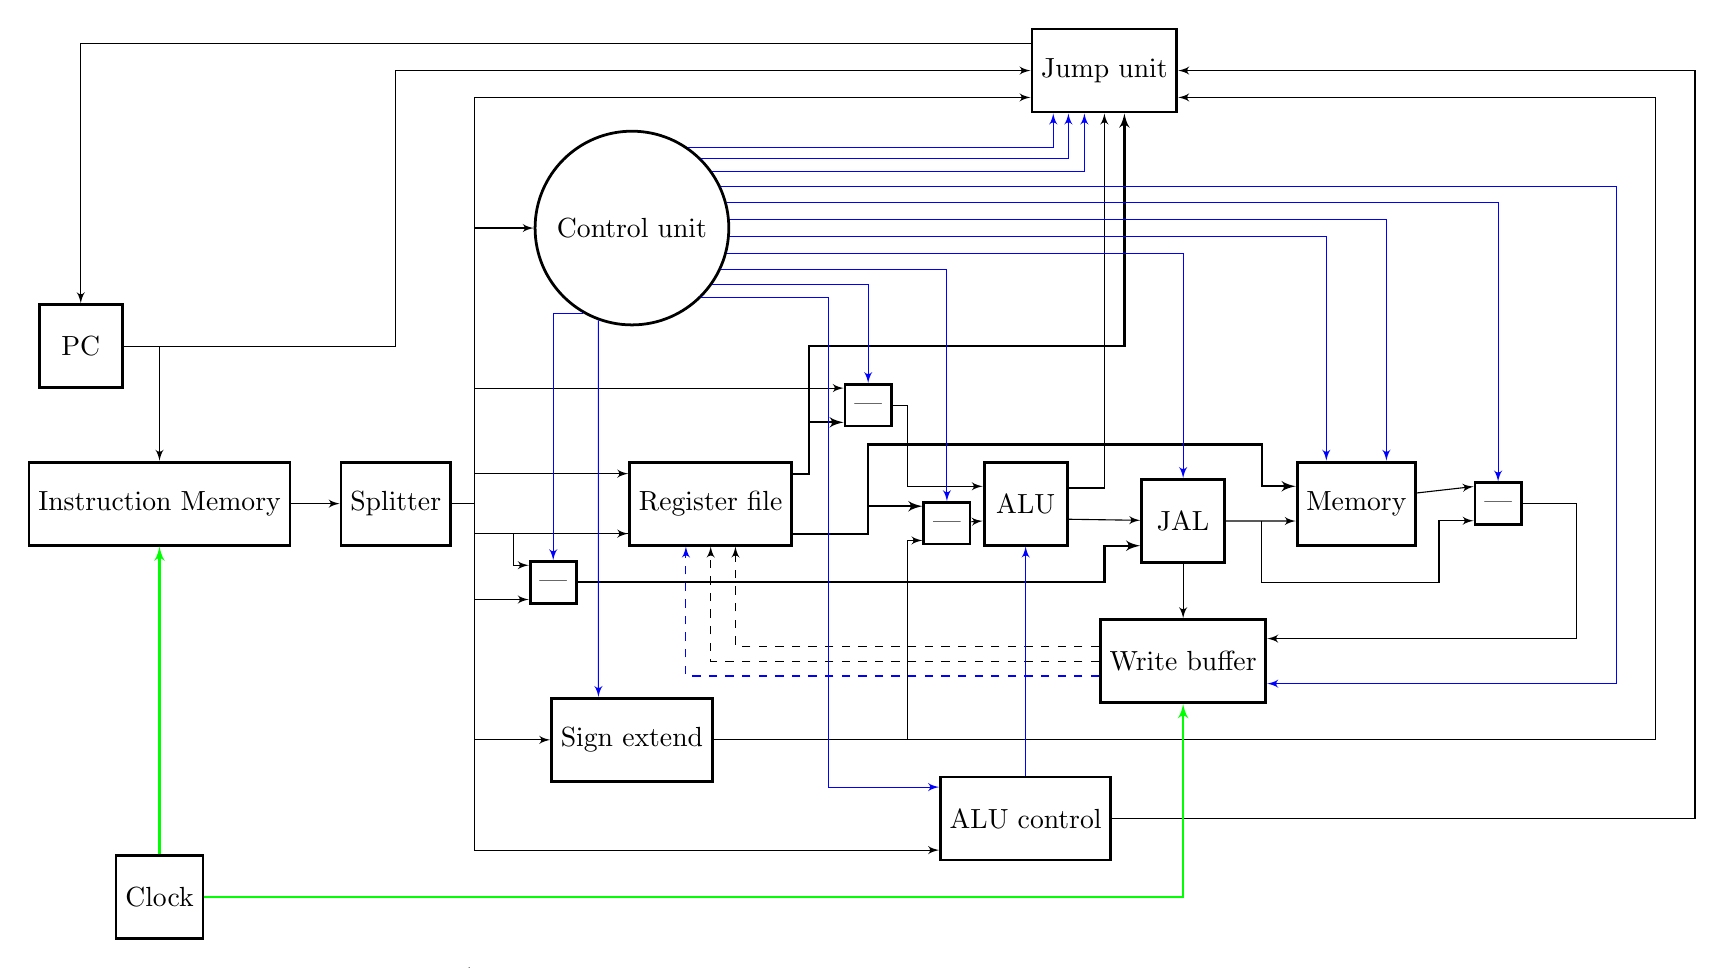
\begin{tikzpicture}
            \node[block] (reg) at (0,0) {Register file};
            \node[control] (cont) at (-1,3.5) {Control unit};
            \node[block] (jump) at (5,5.5) {Jump unit};
            \node[empty] (splitspace) at (-3,0) {};
            \node[block] (split) at (-4,0) {Splitter};
            \node[block] (if) at (-7,0) {Instruction Memory};
            \node[block] (sign) at (-1,-3) {Sign extend};
            \node[block] (alu) at (4,0) {ALU};
            \node[block] (alucont) at (4,-4) {ALU control};
            \node[block] (mem) at (8.2,0) {Memory};
            \node[block] (jal) at (6,-0.22) {JAL};
            \node[mux] (memread) at (10,0) {|};
            \node[mux] (shmt) at (2,1.25) {|};
            \node[mux] (imm) at (3, -0.25) {|};
            \node[mux] (regdst) at (-2,-1) {|};
            \node[block] (pc) at (-8, 2) {PC};
            \node[block] (writebuf) at (6, -2) {Write buffer};

            \path[draw, ->] (if) -- (split);
            \path[draw, -] (split) -- (splitspace.center);
            \path[draw, ->] (splitspace.center) |- (sign);
            \path[draw, ->] (splitspace.center) |- (cont);
            \path[draw, ->] (splitspace.center) |- (reg.160);
            \path[draw, ->] (splitspace.center) |- (reg.200);
            \path[draw, ->] (splitspace.center) |- (jump.200);
            \path[draw, ->] (splitspace.center) |- (alucont.200);
            \path[draw, ->] (splitspace.center) |- (regdst.215);
            \path[draw, ->] (splitspace.center) |- (shmt.145);
            \path[draw, ->] (reg.200) -| (-2.5, -0.5) |- (regdst.145);
            \path[draw, ->] (alucont) -| (12.5, 0) |- (jump);
            \path[draw, thick, ->] (reg.340) -| (2,-0.25) |- (imm.145);
            \path[draw, thick, ->] (2,-0.25) |- (3,0.75) -- (7,0.75) |-
            (mem.164);
            \path[draw, thick, ->] (reg.20) -| (1.25,0.5) |- (shmt.215);
            \path[draw, thick, -] (1.25,0.5) |- (4,2);
            \path[draw, thick, ->] (4,2) -| (jump.295);
            \path[draw, ->] (shmt) -| (2.5, 0.5) |- (alu.158);
            \path[draw, ->] (alu.20) -| (jump);
            \path[draw, ->] (alu.340) -- (jal);
            \path[draw, ->] (jal) -- (mem.196);
            \path[draw, ->] (imm) -- (alu.202);
            \path[draw, ->] (7, -0.22) |- (8, -1) -| (9.25,-0.5) |-
            (memread.215);
            \path[draw, ->] (mem.10) -- (memread.145);
            \path[draw, ->] (sign) -| (2.5, -1) |- (imm.215);
            \path[draw, ->] (2.5,-3) -| (12, 0) |- (jump.340);
            \path[draw, thick, ->] (regdst) -| (5, -0.6) |- (jal.210);
            \path[draw, ->] (pc) -| (if);
            \path[draw, ->] (pc) -| (-4, 4) |- (jump);
            \path[draw, ->] (jump.160) -| (pc);
            \path[draw, ->] (jal) -- (writebuf);
            \path[draw, ->] (memread) -| (11, -1) |- (writebuf.15);
            \path[draw, dashed, ->] (writebuf.170) -| (reg.300);
            \path[draw, dashed, ->] (writebuf) -| (reg);
            \path[draw, dashed, ->, color=blue] (writebuf.190) -| (reg.240);

            \path[draw, ->, color=blue] (alucont) -- (alu);
            \path[draw, ->, color=blue] (cont.55) -| (jump.220);
            \path[draw, ->, color=blue] (cont.45) -| (jump.230);
            \path[draw, ->, color=blue] (cont.35) -| (jump.245);
            \path[draw, ->, color=blue] (cont.25) -| (11.5,0) |-
            (writebuf.345);
            \path[draw, ->, color=blue] (cont.15) -| (memread);
            \path[draw, ->, color=blue] (cont.5) -| (mem.55);
            \path[draw, ->, color=blue] (cont.355) -| (mem.125);
            \path[draw, ->, color=blue] (cont.345) -| (jal);
            \path[draw, ->, color=blue] (cont.335) -| (imm);
            \path[draw, ->, color=blue] (cont.325) -| (shmt);
            \path[draw, ->, color=blue] (cont.315) -| (1.5, 0.5) |-
            (alucont.160);
            \path[draw, ->, color=blue] (cont.250) -- (sign.128);
            \path[draw, ->, color=blue] (cont.240) -| (regdst);

            \node[block] (clock) at (-7, -5) {Clock};
            \path[draw, ->, thick, color=green] (clock) -- (if);
            \path[draw, ->, thick, color=green] (clock) -| (writebuf);
        \end{tikzpicture}
    }
    \caption{Full single cycle MIPS processor. The units with | indicate
    multiplexors. Black wires indicate data wires. Blue wires indicate control
    wires. Green wires indicate clock}
    \label{fig:full}
\end{figure}


%    \item[Jump] Controls whether or not the instruction is a jump instruction,
%        i.e. if the \texttt{PC} register should be changed.

%    \item[JAL] Contrals whether or not the instruction is a \texttt{jal}
%        instruction, i.e. that the \texttt{PC+4} address should be stored.

%    \item[LogicalImmediate] Controls whether or not the sign extender should
%        be a sign extender, in the case of a numeral immediate, or if it
%        should be a zero extender, in the case of a logical I-format
%        instruction.

%\subsection{Jump control}
%The jump control is the part of the processor, that based on the instruction
%changes the value of the PC register. There are two ways to jump: by branching
%and by jumping.
%
%\subsubsection*{Implementation}
%We start by implementing the control for the branching logic. We need to
%support 2 branch instructions in our basic processor: branch equal and branch
%not equal. Therefore we will need two signals: \texttt{Branch} and
%\texttt{BranchNot}. The \texttt{Branch} is used to indicate that the
%instruction should change the PC register. The \texttt{BranchNot} is used to
%choose whether or not the \texttt{Zero} flag from the ALU should be
%\texttt{1} or \texttt{0} for the instruction to branch. In both instructions,
%we compute the subtraction of the two input registers, and if the result is
%\texttt{1} they are equal, otherwise they are not equal. The \texttt{Zero}
%signal is then send to an \texttt{AND} gate along with the \texttt{Branch}
%signal.
%
%Then we need to implement the jump unit. This is a little bit easier, as we do
%not depend on anything from the ALU. The problem is that we need to change the
%decoder to accept a new format: the J-format. The J-format consists of an
%opcode, and a 26-bit address. The address is left shifted by 2, to ensure word
%alignment, and the upper 4 bits of the PC is added to the final address. We
%also need another control signal: \texttt{Jump}. We use this to multiplex
%between the newly computed address and the output from the previous mux (branch
%or pc+4).
%
%\subsubsection*{Testing}
%We test the jump unit by adding jump instructions in the program within the
%Instruction Memory.

%\subsection{Adding additional instructions}
%To add additional instructions, we need to add additional circuitry and entries
%in the \tt{enum}s. We will go through implementing the MIPS core instruction
%set.
%
%We start with the remaining R format instructions (Except for shifting,
%multiplication and division). This is straightforward, as we only need to add
%additional entries to the \tt{enum}s, add the additional cases in the
%\tt{switch} in the ALU control and in the \tt{switch} in the ALU.
%
%For shifting, we need to extract extra information from the instruction in the
%Splitter: the \tt{shamt} field. Following this, we add an additional control
%signal, and multiplex on whether it should be the value read from the registers
%or the \tt{shamt}, which should be the B input for the ALU.
%
%Then we have the remaining arithmetic I format instructions. This is also
%straightforward, as we only need to extend the \tt{enum}s, and add additional
%entries to the \tt{switch} in the ALU control.
%
%Next we need the \tt{jal} instruction. Here we need circuitry to store the
%contents of the \tt{PC} register. To do this, we send the \tt{PC} to the
%\tt{EX} stage, and multiplex on the output from the ALU and the \tt{PC}, with
%the \tt{JAL} control signal.
%
%Next we need the \tt{jr} instruction. We add an additional signal, and
%multiplex on the value read from register, and the normal \tt{PC+4}.
%
%Then we have the \tt{mult}, \tt{multu}, \tt{div} and \tt{divu} instructions.
%These are all R format, so we follow the same procedure. However, instead of
%sending the result on the ALU result bus, we store it in two additional
%registers, which we keep in the ALU: \tt{HI} and \tt{LO}. Following this, we
%can also easily add the instructions \tt{mfhi}, \tt{mflo}, \tt{mthi} and
%\tt{mtlo}, which moves data to and from the two new registers.
%
%Finally, we have the \tt{bne} instruction. We add an additional signal, and
%multiplex the \tt{NOT}ed \tt{zero} signal from the ALU as the signal for the
%branching \tt{AND} gate.
%
%\subsection{Test programs}
%Snak om at bruge MARS!
%
%Now that we have our single cycle MIPS processor, we are ready to throw actual
%instructions at it. We start by collecting all of the smaller test instructions
%into a full test program. SE APPENDIX! (og lav det for den sags skyld)
%
%Then we have a Quicksort written in MIPS assembly.


\newpage
\section{Pipelining}
In this section, we will be looking at pipelining our single cycle MIPS
processor, and handle the problems, which are introduced by pipelining.

We start by going through the background and motivation for pipelining, and
then proceed on how to extend our single cycle MIPS processor to have pipes.

As mentioned, pipelining introduces new problems to handle in the processor,
and we will solve it by adding two new components: the forwarding unit, which
forwards results from previous instructions to later instructions, and the
hazard detection unit, which controls when to stall the pipeline, and when the
instruction should read the forwarded value, or the value stored in the
Register File.

Throughout each step, we will also be writing programs, in order to verify that
our processor behaves as specified.

\subsection{Introducing the pipes}


\subsection{Forwarding}
\subsection{Hazard Detection}


\newpage
%\section{References}
\begin{thebibliography}{9}
    \bibitem{ref:sme} Brian Vinter \& Kenneth Skovhede. \it{Synchronous Message
        Exchange for Hardware Designs}. \copyright\ The authors and Open
        Channel Publishing Ltd. 2014.
    \bibitem{ref:csp} C.A.R. Hoare. \it{Communicating Sequential Processes}.
        \copyright\ ACM 1978
    \bibitem{ref:ark} David A. Patterson \& John L. Hennessy. \it{Computer
        Organization and Design - The Hardware/Software Interface (Revised 4th
        edition)}.  \copyright\ Elsevier 2012
    \bibitem{ref:diku} Maskinarkitektur (ARK) 2013/2014
        \url{http://kurser.ku.dk/course/ndaa04009u/2013-2014}
    \bibitem{ref:logic} Introduction to Combinational Logic Functions
        \url{https://www.allaboutcircuits.com/textbook/digital/chpt-9/combinational-logic-functions/}
\end{thebibliography}



\end{document}
